This chapter describes how subtyping can be used to define quotient-like types. It focuses on issues that may appear while using this approach in Coq and shows how to deal with them.
\section{Subtyping}
\begin{defi}{Subtypes}{def:subtypes}
A \emph{subtype} $A \sqsubseteq B$ is a type that contains a specific subset of elements of the underlying type $B$.
\end{defi}
\begin{example}{}{ex:subtype}
A great example of a subtype is the type of even numbers, which is a subtype of natural numbers.
\end{example}
Subtyping is a pretty intuitive concept. However, subtyping in Coq can confuse users accustomed to object-oriented languages like Java \cite{Java}. In such languages, subtyping is usually associated with the concept of inheritance and is used to define polymorphic construction. In other words, we can use an element of a subtype when an element of the underlying type is required. Similarly, in mathematics, we expect an even number to be a natural number. Unfortunately, such intuitions do not apply in Coq.
\begin{defi}{Subtypes in Coq}{def:siq}
\begin{minted}{coq}
Inductive sig (A : Type) (P : A -> Prop) : Type :=
    exist : forall x : A, P x -> sig P.
\end{minted}
\end{defi}
\begin{defi}{Subtypes in Coq using record}{def:siq'}
\begin{minted}{coq}
Record sig' (A : Type) (P : A -> Prop) : Type := exist' {
    proj1' : A;
    proj2' : P proj1';
}
\end{minted}
\end{defi}
Subtypes in Coq can be defined in two equivalent ways (see definitions \ref{def:siq} and \ref{def:siq'}). The first definition is used in Coq's standard library. The second one nicely shows that a subtype is actually a dependent pair built of two elements -- a value and the proof that the value satisfies a subtype-defining predicate.
\begin{defi}{Depandent pair}{def:dep_pair}
\emph{Dependent pair} is a generalization of a pair where the type of the second element depends on the value of the first one.
\end{defi}
\begin{example}{}{ex:dep_pair}
An example of a dependent pair type is the type of pairs of two coprime numbers. The value of the first element determines the type of the second element. For example, if the first element is five, the second element must be a number coprime to five.
\end{example}
Since subtypes are defined as dependent pairs in Coq, we cannot use an element of the subtype as an element of the underlying type. However, in contrast to the majority of programming languages, in Coq we can use subtypes to define concepts like the type of sorted lists and, for example, use this type as a type of argument of the binary search function. The benefits of such function types are obvious for developing reliable software.
\begin{coq}{The notation for subtyping}{coq:subtype_notation}
In Coq, there is a special notation for subtypes: \mcoq{{a : A | P a}} that should resemble mathematical notation of $\{a \in A: P(a)\}$.
\end{coq}
\begin{example}{The subtype of natural numbers less than 10}{ex:lessThanTen}
\begin{minted}{coq}
Definition lessThanTen := {a : nat | a < 10}.
\end{minted}
\end{example}
\subsection{Connetion to quotient types}
Subtyping is the dual construction of quotient types. As the introduction mentions, there is no built-in method for implementing quotient types in Coq. Therefore, we will use subtypes to define types containing only normalized elements of the underlying type. The normalized elements are defined as the image of some normalization function. This construction defines a type where equality is equivalent to a quotient-defining equality relation because every equivalence class is reduced to a single element.
\begin{defi}{Subtype of normalized elements}{def:subtype_quot}
\begin{minted}{coq}
Record quotient {A : Type} (f : A -> A) `{normalization f} := {
  val         : A;
  valIsNormal : val = f val
}.
\end{minted}
\end{defi}
\section{Duality}
In the previous section, we mentioned that subtyping is a dual concept to quotient types. This optional section explains what it means and why they are considered dual. Knowledge about category theory would improve the reading experience. However, this part is more of an interesting fact than an integral part of this work, so feel free to skip it.
\begin{defi}[]{Duality}{def:dual}
In category theory, the statement \emph{dual} to $\sigma$ is denoted as $\sigma^{\textrm{op}}$ and defined by \cite{CategoryTheory}:
\setlist{nolistsep}
\begin{itemize}
    \itemsep 0em 
    \item interchanging the source and target of each morphism in $\sigma$,
    \item interchanging the order of composing morphisms in $\sigma$.
\end{itemize}
\end{defi}

\begin{vis}[]{Product and coproduct}{vis:dual}
The formal definition of duality might take much effort to understand. A visual example of two dual constructions should give enough insight to comprehend this concept. On the left side, we see a product, and on the right side, a dual construction to product, known as a coproduct.
\begin{center}
    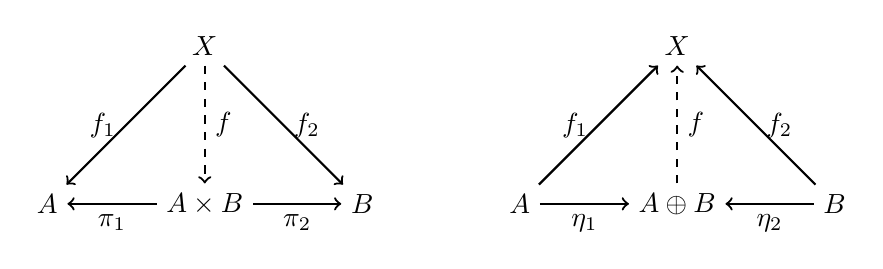
\begin{tikzpicture}[node/.style={circle, draw=black!60, very thick, minimum size=0.4}]
    %Nodes
    \node[] at (0, 0) (pA) {$A$};
    \node[] at (4, 0) (pB) {$B$};
    \node[] at (2, 2) (pX) {$X$};
    \node[] at (2, 0) (pS) {$A \times B$};
    
    \node[] at (6, 0) (cA) {$A$};
    \node[] at (10, 0) (cB) {$B$};
    \node[] at (8, 2) (cX) {$X$};
    \node[] at (8, 0) (cS) {$A \oplus B$};
    
    %Lines
    \draw[->, thick] (pS) -- (pA) node [below, midway] {$\pi_1$};
    \draw[->, thick] (pS) -- (pB) node [below, midway] {$\pi_2$};
    \draw[->, thick] (pX) -- (pA) node [left, midway] {$f_1$};
    \draw[->, thick] (pX) -- (pB) node [right, midway] {$f_2$};
    \draw[->, thick, dashed] (pX) -- (pS) node [right, midway] {$f$};
    
    \draw[->, thick] (cA) -- (cS) node [below, midway] {$\eta_1$};
    \draw[->, thick] (cB) -- (cS) node [below, midway] {$\eta_2$};
    \draw[->, thick] (cA) -- (cX) node [left, midway] {$f_1$};
    \draw[->, thick] (cB) -- (cX) node [right, midway] {$f_2$};
    \draw[->, thick, dashed] (cS) -- (cX) node [right, midway] {$f$};
    
    \end{tikzpicture}
\end{center}
Both diagrams commute, meaning that all directed paths in the diagram with the same start and endpoints lead to the same result \cite{CategoryTheory}.
\end{vis}
In other words, we can construct a dual concept by reversing each arrow (morphism) in the diagram. However, definitions of subtyping and quotient types
do not seem to have any arrows. We must look into pushout and pullback constructions known from category theory \cite{CategoryTheory} to find them.
\subsection{Pushout}
\begin{defi}{Pushout}{def:pusout}
The \emph{pushout} \cite{CategoryTheory} $P$ is defined by two morphisms $f: X \rightarrow A$ and $g: X \rightarrow B$, with common domain $X$.
\begin{center}
    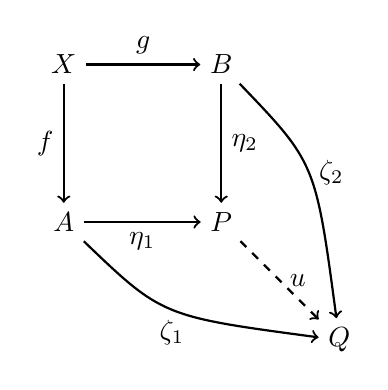
\begin{tikzpicture}[node/.style={circle, draw=black!60, very thick, minimum size=0.4}]
    %Nodes
    \node[] at (0, 0) (a) {$A$};
    \node[] at (2, 0) (p) {$P$};
    \node[] at (0, 2) (x) {$X$};
    \node[] at (2, 2) (b) {$B$};
    
    \node[] at (3.5, -1.5) (q) {$Q$};
    
    %Lines
    \draw[->, thick] (x) -- (a) node [left, midway] {$f$};
    \draw[->, thick] (x) -- (b) node [above, midway] {$g$};
    \draw[->, thick] (a) -- (p) node [below, midway] {$\eta_1$};
    \draw[->, thick] (b) -- (p) node [right, midway] {$\eta_2$};
    \draw[->, thick] (a) .. controls +(1.25, -1.2) .. (q) node [below, midway] {$\zeta_1$};
    \draw[->, thick] (b) .. controls +(1.2, -1.25) .. (q) node [right, midway] {$\zeta_2$};
    \draw[->, thick, dashed] (p) -- (q) node [right, midway] {$u$};
    
    \end{tikzpicture}
\end{center}
The pushout $P$ is an object along with two morphisms $\eta_1: A \rightarrow P$ and $\eta_2: B \rightarrow P$ that complete commutative square with two given morphisms $f: X \rightarrow A$ and $g: X \rightarrow B$. However, not every object that makes the square commutative is a pushout. The pushout must be the "most general" way to complete the commutative square. By the "most general" way, we mean that for every other object Q, which also completes commutative square with two morphisms $\zeta_1: A \rightarrow Q$ and $\zeta_2: B \rightarrow Q$, a unique morphism $u: P \rightarrow Q$ must exist that makes the whole diagram commutative. Not for all morphisms $f: X \rightarrow A$ and $g: X \rightarrow B$, pushout exists, but if it exists, it is unique up to the unique isomorphism.
\end{defi}
The pushout is a useful concept in category theory, but its connection to quotient types is not obvious. To see this connection let us take a trip to the world of \emph{Set} category. In this category, sets are objects, and functions between sets are morphisms. We will show that, indeed, in this category, quotient types are pushouts. On the diagram of the pushout definition, we can see that $A$, $B$, and $P$ define something in the shape of a coproduct. Let us use coproduct $A \oplus B$ as a base for the pushout definition and let functions $\eta_1: A \rightarrow A \oplus B$ and $\eta_2: B \rightarrow A \oplus B$ be natural injections. For $A \oplus B$ to be pushout, we also need to ensure that $X$, $A$, $B$ and $A \oplus B$ create a commutative square, that means for every $x \in X$ following should be true $\eta_1(f(x)) = \eta_2(g(x))$. In order to achieve that, we need to modify $A \oplus B$, by gluing together injections of $f(x)$ and $g(x)$ in $A \oplus B$. As we know, gluing together elements means defining the quotient type $P = ((A \oplus B) / \sim)$, where for every $x \in X$ $f(x) \sim g(x)$. For $P = ((A \oplus B) / \sim)$ to be a pushout, we need to define $(\sim)$ as the largest in terms of the number of equivalence classes relation that completes the commutative square. 
\begin{theo}{}{th:pushout}
If there exists a larger equivalence relation $(\simeq)$ for which  $X$, $A$, $B$, and $Q = ((A \oplus B
)/\simeq)$ also commutes, then there cannot exist a unique morphism $u: P \rightarrow Q$ that makes the whole diagram commutative. 
\end{theo}

\begin{proof}{}{proof:pushout}
Since $|Q| > |P|$, morphism $u$ cannot be a surjection. Therefore,  there exists $y \in Q$ such that for all  $x \in P$ $u(x)$ is not equal to $y$. 
Without loss of generality exists $a \in A$ such that $\zeta_1(a) = y$. From commutivity we know that $\zeta_1(a) = u(\eta_1(a))$, but $\eta_1(a) \in P$. \contradiction
\end{proof}

\begin{example}{Circle defined by a pushout}{ex:circ}
In category \emph{Set}, we can use a pushout to construct a circle out of two bounded lines $[0, 1]$. Let $C$ be a pushout defined by two identity morphisms $\textrm{id}: \{0, 1\} \rightarrow  [0, 1]$.

\begin{center}
    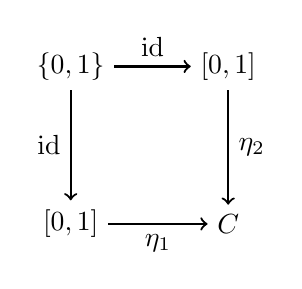
\begin{tikzpicture}[node/.style={circle, draw=black!60, very thick, minimum size=0.4}]
    %Nodes
    \node[] at (0, 0) (a) {$[0, 1]$};
    \node[] at (2, 0) (p) {$C$};
    \node[] at (0, 2) (x) {$\{0, 1\}$};
    \node[] at (2, 2) (b) {$[0, 1]$};
    
    %Lines
    \draw[->, thick] (x) -- (a) node [left, midway] {$\textrm{id}$};
    \draw[->, thick] (x) -- (b) node [above, midway] {$\textrm{id}$};
    \draw[->, thick] (a) -- (p) node [below, midway] {$\eta_1$};
    \draw[->, thick] (b) -- (p) node [right, midway] {$\eta_2$};;
    
    \end{tikzpicture}
\end{center}
Let us check if $C$ is a circle. Since the diagram above commutes, then we know that $\eta_1(0) = \eta_2(0)$ and $\eta_1(1) = \eta_2(1)$ so, we glued together two points. Moreover, we know that $C$ is defined by the largest equivalence relation in terms of equivalence classes. Therefore, every other point of both bounded lines has to have a natural injection into $C$. Based on this, we can conclude that $C$ represents a circle. This construction can be generalized for $n$-dimensional hyper-spheres. Gluing together two $n$-dimensional hemispheres alongside $(n-1)$-dimensional sphere, gives a $n$-dimmensional sphere.
\end{example}

\subsection{Pullback}
Knowing that a pullback is a dual construction to pushout and knowing what dual construction is, everyone should be able to draw a pushout defining diagram.
\begin{defi}{Pullback}{def:pullback}
The pullback \cite{CategoryTheory} $P$ is defined by two morphisms $f: A \rightarrow X$ and $g: B \rightarrow X$, with common codomain $X$.
\begin{center}
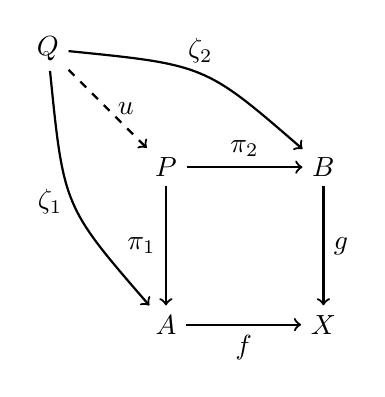
\begin{tikzpicture}[node/.style={circle, draw=black!60, very thick, minimum size=0.4}]
    %Nodes
    \node[] at (0, 0) (a) {$A$};
    \node[] at (0, 2) (p) {$P$};
    \node[] at (2, 0) (x) {$X$};
    \node[] at (2, 2) (b) {$B$};
    
    \node[] at (-1.5, 3.5) (q) {$Q$};
    
    %Lines
    \draw[->, thick] (a) -- (x) node [below, midway] {$f$};
    \draw[->, thick] (b) -- (x) node [right, midway] {$g$};
    \draw[->, thick] (p) -- (a) node [left, midway] {$\pi_1$};
    \draw[->, thick] (p) -- (b) node [above, midway] {$\pi_2$};
    \draw[->, thick] (q) .. controls +(0.2, -2) .. (a) node [left, midway] {$\zeta_1$};
    \draw[->, thick] (q) .. controls +(2, -0.2) .. (b) node [above, midway] {$\zeta_2$};
    \draw[->, thick, dashed] (q) -- (p) node [right, midway] {$u$};
    
    \end{tikzpicture}
\end{center}
The pullback $P$ is an object along with two morphisms $\pi_1: P \rightarrow A$ and $\pi_2: P \rightarrow B$ that complete commutative square with two given morphisms $f: A \rightarrow X$ and $g: B \rightarrow X$. However, not every object that makes the square commutative is a pullback. The pullback must be the "most general" way to complete the commutative square. By the "most general" way, we mean that for every other object Q, which also completes commutative square with two morphisms $\zeta_1: Q \rightarrow A$ and $\zeta_2: Q \rightarrow B$, a unique morphism $u: Q \rightarrow P$ must exist that makes the whole diagram commutative. Not for all morphisms $f: A \rightarrow X$ and $g: B \rightarrow X$, pullback exists, but if it exists, it is unique up to the unique isomorphism.
\end{defi}
To understand the connection between a pullback and subtyping, we take a trip to the \emph{Set} category again. As expected in dual construction, in the pullback $A$, $B$, and $P$ are in the shape of a product. Therefore, let us use product $A \times B$ as the base for the pushout definition and let functions $\pi_1: A \times B \rightarrow A$ and $\pi_2: A \times B \rightarrow B$ be natural projections. In order to complete the commutative square for every $p \in A \times B$, the following needs to be true $f (\pi_1 (p)) = g (\pi_2(p))$. Therefore, we need to use the following subset $P = \{(a, b) \in A \times B : f(a) = g(b)\}$. 
\begin{theo}{}{th:pulback}
For every other subset $Q \subseteq A \times B$ and two morphisms $\zeta_1: Q \rightarrow A$ and $\zeta_1: Q \rightarrow B$ that complete the commutative square, there exists a unique morphism $u: Q \rightarrow P$, which makes the whole diagram commutative.
\end{theo}
\begin{proof}{}{proof:pullback}
Let define $u(q) = (\zeta_1(q), \zeta_2(q))$. Since $\pi$ functions are simple projections the following is true $\zeta_1 = \pi_1 \circ u$ and $\zeta_2 = \pi_2 \circ u$. \qed
\end{proof}
\begin{example}{Pairs of integers with the same parity}{ex:parity_pair}
In category \emph{Set}, we can use the pullback to define the set of pairs of integers with the same parity. Let us define morphism $f(n) = n \; \textrm{mod} \; 2$ that checks the parity of an integer.
\begin{center}
    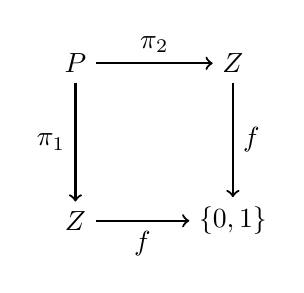
\begin{tikzpicture}[node/.style={circle, draw=black!60, very thick, minimum size=0.4}]
    %Nodes
    \node[] at (0, 0) (a) {$\mathbb{Z}$};
    \node[] at (0, 2) (p) {$P$};
    \node[] at (2, 0) (x) {$\{0, 1\}$};
    \node[] at (2, 2) (b) {$\mathbb{Z}$};
    
    %Lines
    \draw[->, thick] (a) -- (x) node [below, midway] {$f$};
    \draw[->, thick] (b) -- (x) node [right, midway] {$f$};
    \draw[->, thick] (p) -- (a) node [left, midway] {$\pi_1$};
    \draw[->, thick] (p) -- (b) node [above, midway] {$\pi_2$};;
    
    \end{tikzpicture}
\end{center}
As we know, the "most general" $P$ that completes this commutative square is $\{(n, m) \in \mathbb{Z} \times \mathbb{Z} : n \equiv_2 m\}$.
\end{example}
\subsection{Conclusion}
As shown in the examples above, the pushout can define quotient types in category theory, and the pullback can be used to define subtypes.  Those two constructions are mutually dual. Therefore, we can call subtyping a dual concept to quotient types.
\section{Uniqueness of representation}
In Coq, subtyping is accomplished by using dependent pairs of value and proof that the value satisfies the subtype-defining predicate. Unfortunately, this means that only some properties of subtypes known from mathematics hold in Coq. As it was mentioned at the beginning of this chapter, we cannot use a member of a subtype as a member of the underlying type. This particular problem is easy to fix using projections. The other consequence of using dependent pairs related to using subtyping as quotient-like types is that we cannot prove that only one member of the subtype exists for every value that satisfies the normalization predicate. As we know, the irrelevance of proofs is independent of the axioms of the \mcoq{Prop} sort \cite{CoqBook2}. It is a major problem since we want to use subtyping to reduce each equivalence class to a single element. The possibility of the existence of multiple elements that only differ by proof of subtype defining predicate makes this construction useless for quotient types applications. Hence, we need to define the subset of quotient types for which its subtype representations are unique or redefine this construction for these purposes.
\begin{defi}{Class of subtypes with unique represenations}{def:unique_representation}
\begin{minted}{coq}
Class unique_representation {A : Type} (P : A -> Prop) := 
  uniq : forall (x y : {a : A | P a}), proj1_sig x = proj1_sig y 
           -> x = y.
\end{minted}
\end{defi}
\begin{coq}{}{coq:proj1_sig}
In Coq function \mcoq{proj1_sig} is a projection of the subtype value. It can be thought of as a lifting to the underlying type.
\end{coq}
\subsection{Axiomatic approach}
As mentioned in the introduction, we avoid using axioms in this paper. However, it is worth considering their effect on the uniqueness of representstion problem and whether using them is safe.
\subsubsection{Proof irrelevance axiom}
Proof irrelevance is a known concept in computer science \cite{ProofIrrelevance}. It states that every two proofs of the same statement are equal.
\begin{defi}{Axiom of proof irrelevance}{def:proof_irrelevance}
\begin{minted}{coq}
Definition Irrelevance := forall (P : Prop) (x y : P), x = y.
\end{minted}
\end{defi}
Using this axiom, we can easily prove that every subtype has a unique representation (as defined in \ref{def:unique_representation}).
\begin{theo}{}{th:irr_uniq}
    \begin{minted}{coq}
Theorem irrelevance_impl_unique_representation : Irrelevance -> 
  forall (A : Type) (P : A -> Prop), unique_representation P.
    \end{minted}
\end{theo}
\begin{proof}{}{proof:irr_uniq}
    \begin{minted}{coq}
intros Irr A P. constructor. intros [x xp] [y yp] H.
cbn in H. subst.
Require Import Coq.Logic.EqdepFacts.
apply eq_dep_eq_sig.
specialize (Irr (P y) xp yp); subst.
constructor. Qed.
\end{minted}
\end{proof}
Those two statements are equivalent. Thus, the axiom of proof irrelevance is required for every subtype to have a unique representation.
\begin{theo}{}{th:irr_uniq2}
    \begin{minted}{coq}
Theorem unique_representation_impl_irrelevance : 
  (forall (A : Type) (P : A -> Prop), unique_representation P) -> 
  Irrelevance.
    \end{minted}
\end{theo}
\begin{proof}{}{proof:irr_uniq2}
    \begin{minted}{coq}
intros Uniq P x y.
specialize (Uniq unit (fun _ => P)). destruct Uniq as [Uniq].
specialize (Uniq (exist _ tt x) (exist _ tt y) eq_refl).
Require Import Coq.Logic.Eqdep_dec.
refine (eq_dep_eq_dec (A := unit) _ _).
- intros. left. destruct x0, y0. reflexivity.
- apply eq_sig_eq_dep. apply Uniq. Qed.
\end{minted}
\end{proof}
\begin{coq}{Dependent equality}{coq:eq_dep}
In coq, \emph{dependent equality} is defined as:
\begin{minted}{coq}
Inductive eq_dep (U : Type) (P : U -> Type) (p : U) (x : P p) 
  : forall q : U, P q -> Prop :=
    eq_dep_intro : eq_dep U P p x p x.
\end{minted}
Proofs above use additional theorems, \mcoq{eq_dep_eq_sig} state that if two values are dependently equal, then subtypes made of them are equal. The second one, \mcoq{eq_sig_eq_dep}, states that for types with decidable equality, dependent equality implies equality.
\end{coq}

\subsubsection{Axiom K}
Axiom K (also known as Uniqueness of Identity Proof) is a weaker version of the proof irrelevance axiom. It states that two proofs of the same equality are equal. Thomas Streicher first introduced it in his habilitation thesis \cite{Streicher}.
\begin{defi}{Axiom K}{def:axiom_K}
\begin{minted}{coq}
Definition K := forall (A : Type) (x y : A) (p q : x = y), p = q.
\end{minted}
\end{defi}
\begin{coq}{Embedding dependent equality in equality}{coq:eq_emb}
An interesting consequence of using axiom K is that it embeds dependent equality in equality.
\begin{minted}{coq}
Fact eq_dep_embedded_in_eq : forall (A : Type) (P : A -> Prop)
  (a : A) (p q : P a), eq_dep A P a p a q -> p = q.
\end{minted}
Moreover, this fact is equivalent to axiom K. Proofs of these facts are outside the scope of this section, but they can be found in \coqsource{Extras/Stricher.v}.
\end{coq}
Since axiom K is weaker than the proof irrelevance axiom, we cannot prove that every subtype has unique representations. However, we can use it to prove that every quotient-like type (defined in \ref{def:subtype_quot}) has unique representations as defined in \ref{def:unique_representation}.
\begin{theo}{}{th:subtype_quot_uniq}
\begin{minted}{coq}
Theorem quotient_unique_representation : K -> forall (A : Type) 
  (f : A -> A) `{normalization A f} (x y : quotient f),
  val x = val y -> x = y.
\end{minted}
\end{theo}
\begin{proof}{}{proof:subtype_quot_uniq}
\begin{minted}{coq}
intros K A f N [x xp] [y yp] H. 
cbn in *. subst. 
specialize (K _ _ _ xp yp). subst. 
reflexivity. Qed.
\end{minted}
\end{proof}
\subsection{Definitional irrelevance approach}
As it was mentioned in this section, we can add the axiom of proof irrelevance to solve the problem of unique representations for every subtype. In Coq, there is another approach to proof irrelevance -- \mcoq{SProp}.
\begin{coq}[]{\mcoq{SProp} sort}{coq:SProp}
\mcoq{SProp} (Strict Propositions) is a sort of propositions with definitional proof irrelevance as described in \cite{BasesOfSProp}. It is still an experimental feature \cite{coqDoc} of Coq and requires work to be fully functional. That said, The standard library of Coq has several useful constructions for strict propositions:
\begin{description}
    \item \mcoq{Box} -- a record that lifts \mcoq{SProp} proposition to \mcoq{Prop} sort.
    \begin{minted}{coq}
Record Box (A : SProp) : Prop := box { unbox : A }.
    \end{minted}
    \item \mcoq{Squash} -- an inductive type that squashes proposition into \mcoq{SProp} sort making it proof irrelevant.
    \begin{minted}{coq}
Inductive Squash (A : Type) : SProp :=  
  squash : A -> Squash A.
    \end{minted}
    \item \mcoq{sEmpty} -- an equivalent of \mcoq{False} in \mcoq{Prop}. From \mcoq{sEmpty} any proposition follows.
    \begin{minted}{coq}
Inductive sEmpty : SProp := .
Definition sEmpty_rect : forall (P : sEmpty -> Type) 
  (s : sEmpty), P s.
    \end{minted}
    \item \mcoq{sUnit} -- an equivalent of \mcoq{True} in \mcoq{Prop}.
    \begin{minted}{coq}
Inductive sUnit : SProp := stt : sUnit.
    \end{minted}
    \item \mcoq{Ssig} -- subtype defined in \mcoq{SProp} sort.
    \begin{minted}{coq}
Record Ssig (A : Type) (P : A -> SProp) : Type :=
  Sexists { Spr1 : A;  Spr2 : P Spr1 }.
    \end{minted}
\end{description}
\end{coq}
We can easily prove that subtypes defined using \mcoq{Ssig} have unique representations.
\begin{theo}{}{th:ssig}
\begin{minted}{coq}
Theorem Ssig_unique_representation : forall (A : Type) 
  (P : A -> SProp) (a b : Ssig P), Spr1 a = Spr1 b -> a = b.
\end{minted}
\end{theo}
\begin{proof}{}{proof:ssig}
\begin{minted}{coq}
intros A P [a ap] [b bp] H.
cbn in *. subst.
reflexivity. Qed.
\end{minted}
\end{proof}
Using \mcoq{Ssig} is very convenient since having unique representations does not require additional axioms. However, the disadvantage of this approach is that the proof that the value satisfies the subtype defining predicate is in the \mcoq{SProp} sort. Therefore, using this proof in the \mcoq{Prop} sort, where most theorems live, is usually impossible. The only exception is when we can use it to prove \mcoq{sEmpty}.
\subsection{Homotopic approach}
If we want to work in the \mcoq{Prop} sort without additional axioms, we must find underlying types with unique identity poofs. It is a challenging task. Nevertheless, with help comes homotopy type theory (HoTT) \cite{HoTT}. It is a relatively new branch of type theory focusing on identity proofs. Homotopic interpretation of a type is $\omega$-grupoid. In such groupoid, nodes represent members of a type; paths represent identity proofs; paths between paths represent identity proofs of identity proofs, and so forth. 
\subsubsection{Homotopy $n$-types}
Homotopy $n$-types creates a type hierarchy based on the complexity of identity poofs structure ($\omega$-grupoid structure).
\begin{example}{Selected $n$-types}{ex:n_types}
Developing intuition regarding this concept is important before formally defining the $n$-th type. Therefore, we will discuss the three most important examples of $n$-types (universes) in this thesis.
\begin{description}
    \item \mcoq{Contr} -- it is the lowest minus-second universe. The type that lives in \mcoq{Contr} has exactly one element. A good example of $(-2)$-type is a \mcoq{unit}.
    \begin{minted}{coq}
 Class isContr (A : Type) := ContrBuilder {
   center : A;
   contr  : forall x : A, x = center
 }.
    \end{minted}
    \item \mcoq{HProp} -- it is the minus-first universe. Not to be confused with Coq's \mcoq{Prop}. The type that lives in it has every element equal to each other. A good example of $(-1)$-type is \mcoq{Empty_set}. We can easily prove that each element of the empty type is the same element. However, it has no elements, so it cannot live in \mcoq{Contr}.
        \begin{minted}{coq}
 Class isHProp (P : Type) :=
   hProp : forall p q : P, p = q.
    \end{minted}
    \item \mcoq{HSet} -- it is the zero universe. Not to be confused with Coq's \mcoq{Set}. The type that lives in it has unique identity proofs. A good example of $0$-type is \mcoq{boo}l. Later in this section we will show that it has unique identity proofs. Moreover, it has two elements, so it does not live in \mcoq{HProp}.
    \begin{minted}{coq}
 Class isHSet (X : Type) :=
   hSet : forall (x y : X) (p q : x = y), p = q.
    \end{minted}
\end{description}
\end{example}
\begin{defi}{$N$-th type}{def:nth_type}
\begin{minted}{coq}
Inductive universe : Type :=
| minus_two  : universe
| S_universe : universe -> universe.

Fixpoint isNType (n : universe) (A : Type) : Type :=
match n with
| minus_two     => isContr A
| S_universe n' => forall x y : A, isNType n' (x = y)
end.
\end{minted}
\end{defi}
As we see in the definition, $n$-types are defined by where identity proofs of elements of those types live. The hierarchy starts at the $(-2)$-type, where only the most primitive contactable types live. Types with identity proofs in \mcoq{Contr} live in \mcoq{HProp} since the identity proof type is inhabited for every pair of elements. Therefore, every two elements are equal. Similarly, if identity proofs of type live in \mcoq{HProp}, then the type lives in \mcoq{HSet} since one or no identity proof exists for every two elements of an underlying type. The other important fact is that every $n$-type is also a $(n+1)$-type.
\begin{theo}{$n$-type inclusion}{th:nth_incl}
\begin{minted}{coq}
Theorem NType_inclusion : forall A: Type, forall n : universe,
  isNType n A -> isNType (S_universe n) A.
\end{minted}
\end{theo}
\begin{proof}{}{proof:nth_incl}
Proof of this theorem can be found in \coqsource{Lib/HoTT.v}.
\end{proof}
\subsubsection{Types with decidable equality}
If the underlying type of quotient-like type (defined in \ref{def:subtype_quot}) lives in the \mcoq{HSet} universe, then we can easily prove that it has a unique representation the same way as in proof \ref{proof:subtype_quot_uniq}. However, proving that a type lives in \mcoq{HSet} is not trivial. Fortunately, Hedberg's theorem \cite{hedberg_1998} gives us a valuable sufficiency condition for being \mcoq{HSet} -- decidable equality.
\begin{defi}{Decidable equality}{def:dec_eq}
\begin{minted}{coq}
Class Decidable (A : Type) :=
  dec : A + (A -> False).
  
Class DecidableEq (A : Type) :=
  dec_eq : forall x y: A, Decidable (x = y).
\end{minted}
\end{defi}
For a type to have decidable equality means that there exists an algorithm that, in a finite amount of time, decides if two elements of this type are equal.
\begin{theo}{Hedberg's theorem}{th:hedberg}
\begin{minted}{coq}
Theorem hedberg (A : Type) : EqDec A -> isHSet A.
\end{minted}
\end{theo}
\begin{proof}{}{proof:hedberg}
This proof of Hedberg's theorem is based on the paper \cite{HedbergProof}. It uses the concept of collapsibility.
\begin{minted}{coq}
Class Collapsible (A : Type) := { 
  collapse        : A -> A ;
  wconst_collapse : forall x y: A, collapse x = collapse y;
}.
\end{minted}
It can be easily proven that the type is collapsible if it is decidable.
\begin{minted}{coq}
Theorem dec_is_collaps : forall A : Type, Decidable A -> 
  Collapsible A.
Proof.
  intros A eq. destruct eq.
  - exists (fun x => a). intros x y. reflexivity.
  - exists (fun x => x); intros x y.
    exfalso; apply f; assumption.
Qed.
\end{minted}
The same law applies to the type of identity proofs.
\begin{minted}{coq}
Class PathCollapsible (A : Type) :=
  path_coll : forall (x y : A), Collapsible (x = y).

Theorem eq_dec_is_path_collaps : forall A : Type, 
  DecidableEq A -> PathCollapsible A.
Proof.
  intros A dec x y. apply dec_is_collaps. apply dec.
Qed.
\end{minted}
We need a simple lemma about composition identity proofs.
\begin{minted}{coq}
Lemma loop_eq : forall A: Type, forall x y: A, forall p: x = y, 
  eq_refl = eq_trans (eq_sym p) p.
Proof.
  intros A x y []. cbn. reflexivity.
Qed.
\end{minted}
Using the lemma above, we can prove that type with collapsable paths lives in \mcoq{HSet}.
\begin{minted}{coq}
Theorem path_collaps_is_hset (A : Type) : PathCollapsible A -> 
  isHSet A.
Proof.
  unfold isHSet, PathCollapsible; intros C x y.
  cut (forall e : x = y, e = 
    eq_trans (eq_sym (collapse (eq_refl x))) (collapse e)).
  - intros H p q. 
    rewrite (H q), (H p), (wconst_collapse p q).
    reflexivity.
  - intros []. apply loop_eq.
Qed.
\end{minted}
Composing \mcoq{dec_is_collaps} with \mcoq{path_collaps_is_hset}, we get proof that every type with decidable equality lives in \mcoq{HSet} and has only trivial paths. \qed
\end{proof}
Hedberg's theorem shows that every quotient-like type (defined in \ref{def:subtype_quot}) with an underlying type with decidable equality has unique representations. However, most types with normalization functions (defined in \ref{def:normalization_function}) have decidable equality.
\subsubsection{$n$-types of function types}
It is also worth characterizing $n$-type of function type based on the $n$-type of its domain and codomain. To do this, we first need to define homotopic equivalence. 
\begin{defi}{Homotopic equivalence}{def:HEquiv}
\begin{minted}{coq}
Class HEquiv (A B : Type) := {
  izo     : A -> B;
  inv     : B -> A ;
  eisretr : forall b : B, izo (inv b) = b;
  eissect : forall a : A, inv (izo a) = a;
  eisadj  : forall a : A, eisretr (izo a) = ap izo (eissect a);
}.
\end{minted}
\end{defi}
The last element of equivalence \mcoq{eisadj} is required for the equivalence type to live in \mcoq{HProp}. This property, however, is not required for this thesis. Therefore, we will skip it, for interested it can be found in \cite{HoTT}. Proof that this is an equivalence relation can be found in \coqsource{Lib/HoTT.v}. Since we are working with functions, we need an axiom of functional extensionality.
\begin{defi}{Homotopic functional extensionality}{def:HFunExt}
\begin{minted}{coq}
Definition happly {A : Type} {B : A -> Type} 
  {f g : forall x : A, B x} (p : f = g) (x : A) : f x = g x :=
  match p with
  | eq_refl => eq_refl
  end.

Definition HFunExt : Type := forall (A : Type) (B : A -> Type) 
  (f g : forall a : A, B a), IsEquiv (happly (f := f) (g := g)).
\end{minted}
\end{defi}
This definition of functional extensionality is perfect for homotopic reasoning since it uses the homotopic equivalence definition \ref{def:HEquiv}. Using these tools, we can characterize $n$-type of function types. The $n$-type of function type depends solely on the $n$-type of the codomain. 
\begin{theo}{$n$-type of function type}{th:fun_is_img_level}
\begin{minted}{coq}
Theorem fun_is_img_level (A B : Type) (n : universe) 
  (funExt : HFunExt) : isNType n B -> isNType n (A -> B).
\end{minted}  
\end{theo}
\begin{proof}{}{proof:fun_is_img_level}
For \mcoq{HProp}, we can prove this theorem.
\begin{minted}{coq}
Lemma fun_is_img_hprop (A : Type) (B : A -> Type) 
  (funExt : HFunExt) : (forall a : A, isHProp (B a)) -> 
  isHProp (forall a : A, B a).
Proof.
  unfold isHProp. intros H f g. 
  destruct (F A B f g) as (inv, _, _, _). apply inv. 
  intros x; apply H.
Qed.
\end{minted} 
We can also prove this for \mcoq{Contr}.
\begin{minted}{coq}
Lemma fun_is_img_contr (A : Type) (B : A -> Type) 
  (funExt : HFunExt) : (forall a : A, isContr (B a)) -> 
  isContr (forall a : A, B a).
Proof.
  assert (C' : forall T: Type, T * (isHProp T) -> isContr T).
  { intros T (c, hprop). exists c. intros t. apply hprop. }
  intros H. apply C'. split.
  - intros a. destruct (H a). assumption.
  - apply fun_is_img_hprop; [auto |].
    intros a b b'.
    destruct (H a) as (c, l).
    rewrite (l b), (l b'). auto. 
Qed. 
\end{minted} 
We need the following theorem about $n$-type of equivalent types to prove this theorem. 
\begin{minted}{coq}
Theorem equiv_keep_level (A B : Type) (n : universe) :
   isNType n A -> Equiv B A -> isNType n B.
\end{minted} 
Proof of this lemma is outside of the scope of this section. However, it can be found in \coqsource{Lib/HoTT.v}. Now we can prove this fact for dependent functions.
\begin{minted}{coq}
Lemma fun_is_img_level_dep (A : Type) (B : A -> Type) 
  (n : universe) (funExt : HFunExt) : 
  (forall a: A, isNType n (B a)) -> isNType n (forall a: A, B a).
Proof.
  revert A B. induction n; intros A B H; cbn in *.
  - apply fun_is_img_contr; auto.
  - intros f g. 
    apply (equiv_keep_level (forall x : A, f x = g x)).
    + apply IHn. intros a. apply H.
    + destruct (funExt A B f g) as (inv, rets, sect, adj).
      econstructor; econstructor; apply adj.
Qed.
\end{minted}
Since our theorem is a particular case of the above lemma, we consider the theorem to be proved. \qed
\end{proof}
\subsubsection{Characterization of dependent pair equality}
\begin{coq}{Dependent pair}{coq:dep_pair}
In Coq, the type of \emph{dependant pair} is defined using inductive type.
\begin{minted}{coq}
Inductive sigT (A : Type) (P : A -> Type) : Type :=
  existT : forall x : A, P x -> sigT A P.
\end{minted}
\mcoq{{x : A & P x}} is the notation for dependent pairs.
\end{coq}
Subtypes are based on dependent pairs. Therefore, knowing how the equality of dependent pairs can be characterized is beneficial. In the case of simple non-dependent pairs, the characterization is straightforward.
\begin{theo}{Characterization of pair equality}{th:pair_eq}
\begin{minted}{coq}
Theorem pair_eq : forall (A B : Type) (a x : A) (b y : B),
  (a, b) = (x, y) -> a = x /\ b = y.
\end{minted}
\end{theo}
\begin{proof}{}{proof:pair_eq}
\begin{minted}{coq}
intros. inversion H. split; trivial. Qed.
\end{minted}
\end{proof}
Using the same definition for dependent pairs is impossible. The first issue is the error of ill-defined equality since \mcoq{P x} and \mcoq{P y} differ in the Coq type system, even if \mcoq{x = y}, and elements of two different types cannot be in equality relation. Even if we change our problem to the characterization of equality for dependent pairs with the same first element, it is still impossible to characterize it using simple equality. Such equality can be characterized using dependent equality known from fact \ref{coq:eq_dep}. Moreover, that characterization using simple equality is correct only if dependent equality is equivalent to equality. From fact \ref{coq:eq_emb}, we know that it is true if and only if axiom K is true. To characterize the general case of dependent pairs equality, we must first define the transport along an equality path.
\begin{defi}{Transport}{def:transport}
\begin{minted}{coq}
Definition transport {A : Type} {a b : A} {P : A -> Type} 
  (p : a = b) (x : P a) : P b :=
match p with
| eq_refl => x
end.
\end{minted}
\end{defi}
Transport construction moves an element of type \mcoq{P a} to a new type  \mcoq{P b} along the path (proof of equality) \mcoq{p: a = b}. Using this construction, we can characterize equality of dependent pairs.
\begin{vis}[G]{Transport}{vis:transport}
$P$ is a family of types indexed by elements of type $A$. Two elements, $a$ and $b$, are equal in $A$, and $p$ is a proof of this fact (path). Element $x$ of type $P(a)$ can be transported along this proof (path) to type $P(b)$.
\begin{center}
\begin{tikzpicture}
    \draw (0,0) circle [x radius=5cm, y radius=1cm];
    \fill (5, -1) circle (0pt) node[above, scale=1.5] {$A$};
    \draw (-4,3) circle [x radius=2cm, y radius=1.2cm, rotate=10];
    \fill (-2.7,4.2) circle (0pt) node[above, right,scale=1.5] {$P(a)$};
    \draw (4,3) circle [x radius=2cm, y radius=1.2cm, rotate=-10];
    \fill (2.7,4.2) circle (0pt) node[above, left,scale=1.5] {$P(b)$};
    \draw [line width=1pt, double distance=7pt,
             arrows = {-Stealth[length=20pt, inset=11pt, width=22pt]}] (4,0.2) -- (4,1.6) node[midway, right=3mm]{$P$};
    \draw [line width=1pt, double distance=7pt,
             arrows = {-Stealth[length=20pt, inset=11pt, width=22pt]}] (-4,0.2) -- (-4,1.6) node[midway, left=3mm]{$P$};
    
    
    \fill (4,0) circle (2pt) node[right] {$b$};
    \fill (-4,0) circle (2pt) node[left] {$a$};
    \draw[dashed] (-4,0)  to [out=45,in=-135,looseness=0.3] (4,0) node[midway, above=3pt]{$p$: $a =_A b$};
    
    \fill (-3.2,2.8) circle (2pt) node[left] {$x$};
    \fill (3.2,2.8) circle (2pt) node[right] {$\textrm{transport}_p(x)$};
    
    \draw [-{Stealth[length=3mm]}] (-3.2,2.8) to [out=45,in=135,looseness=0.6] (3.1,2.9);
    
\end{tikzpicture}
\end{center}
\end{vis}
\begin{theo}{Characterization of dependent pair equality}{th:dep_pair_eq}
\begin{minted}{coq}
Theorem dep_pair_eq : forall (A : Type) (P : A -> Type) 
  (x y : A) (p : P x) (q : P y), existT P x p = existT P y q ->
  exists e : x = y, transport e p = q.
\end{minted}
\end{theo}
\begin{proof}{}{proof:dep_pair_eq}
\begin{minted}{coq}
intros A P x y p q H. inversion H.
exists eq_refl. cbn. trivial. Qed.
\end{minted}
\end{proof}